\documentclass[a4paper]{book}
\usepackage{a4wide}
\usepackage{makeidx}
\usepackage{fancyhdr}
\usepackage{graphicx}
\usepackage{multicol}
\usepackage{float}
\usepackage{textcomp}
\usepackage{alltt}
\usepackage{times}
\usepackage{ifpdf}
\ifpdf
\usepackage[pdftex,
            pagebackref=true,
            colorlinks=true,
            linkcolor=blue,
            unicode
           ]{hyperref}
\else
\usepackage[ps2pdf,
            pagebackref=true,
            colorlinks=true,
            linkcolor=blue,
            unicode
           ]{hyperref}
\usepackage{pspicture}
\fi
\usepackage[utf8]{inputenc}
\usepackage{doxygen}
\makeindex
\setcounter{tocdepth}{3}
\renewcommand{\footrulewidth}{0.4pt}
\begin{document}
\begin{titlepage}
\vspace*{7cm}
\begin{center}
{\Large Nessie, reconocedor óptico de texto en recortes de prensa escrita \\[1ex]\large 1.0 }\\
\vspace*{1cm}
{\large Generated by Doxygen 1.5.6}\\
\vspace*{0.5cm}
{\small Mon Sep 22 20:25:28 2008}\\
\end{center}
\end{titlepage}
\clearemptydoublepage
\pagenumbering{roman}
\tableofcontents
\clearemptydoublepage
\pagenumbering{arabic}
\chapter{Directory Hierarchy}
\section{Directories}
This directory hierarchy is sorted roughly, but not completely, alphabetically:\begin{CompactList}
\item \contentsline{section}{inc}{\pageref{dir_ef15eccf5bd9eca446a41a18c57ac0fd}}{}
\item \contentsline{section}{src}{\pageref{dir_f108b8e716a38a781a23bf0e62a4b450}}{}
\end{CompactList}

\chapter{Data Structure Index}
\subsection{Data Structures}
Here are the data structures with brief descriptions:\begin{CompactList}
\item\contentsline{section}{\hyperlink{class_clip}{Clip} (Press clip where the recognizer has to extract the text from )}{\pageref{class_clip}}{}
\item\contentsline{section}{\hyperlink{class_clip_location}{ClipLocation} (Location of a press clip inside a newspaper page )}{\pageref{class_clip_location}}{}
\item\contentsline{section}{\hyperlink{class_nessie_exception}{NessieException} (Exception raised by a Nessie OCR object )}{\pageref{class_nessie_exception}}{}
\item\contentsline{section}{\hyperlink{class_preprocessor}{Preprocessor} (\hyperlink{class_preprocessor}{Preprocessor} of the OCR process )}{\pageref{class_preprocessor}}{}
\item\contentsline{section}{\hyperlink{class_recognizer}{Recognizer} (Manager of the whole OCR process )}{\pageref{class_recognizer}}{}
\item\contentsline{section}{\hyperlink{class_segmenter}{Segmenter} (\hyperlink{class_segmenter}{Segmenter} of the OCR process )}{\pageref{class_segmenter}}{}
\item\contentsline{section}{\hyperlink{class_shape}{Shape} (The shape of a character in a press clip )}{\pageref{class_shape}}{}
\item\contentsline{section}{\hyperlink{class_statistics}{Statistics} (Statistical data regarding the text recognition process )}{\pageref{class_statistics}}{}
\item\contentsline{section}{\hyperlink{class_text}{Text} (\hyperlink{class_text}{Text} extracted by the recognizer )}{\pageref{class_text}}{}
\end{CompactList}

\chapter{File Index}
\section{File List}
Here is a list of all documented files with brief descriptions:\begin{CompactList}
\item\contentsline{section}{\textbf{Classifier.cpp} }{\pageref{_classifier_8cpp}}{}
\item\contentsline{section}{\textbf{Classifier.h} }{\pageref{_classifier_8h}}{}
\item\contentsline{section}{\hyperlink{_clip_8cpp}{Clip.cpp} (Implementation of class \hyperlink{class_clip}{Clip} )}{\pageref{_clip_8cpp}}{}
\item\contentsline{section}{\hyperlink{_clip_8h}{Clip.h} (Declaration of class \hyperlink{class_clip}{Clip} )}{\pageref{_clip_8h}}{}
\item\contentsline{section}{\hyperlink{_colorspace_8h}{Colorspace.h} (Declaration of enumeration Colorspace )}{\pageref{_colorspace_8h}}{}
\item\contentsline{section}{\textbf{FeatureVector.cpp} }{\pageref{_feature_vector_8cpp}}{}
\item\contentsline{section}{\textbf{FeatureVector.h} }{\pageref{_feature_vector_8h}}{}
\item\contentsline{section}{\textbf{loadPDF.cpp} }{\pageref{load_p_d_f_8cpp}}{}
\item\contentsline{section}{\textbf{main.cpp} }{\pageref{main_8cpp}}{}
\item\contentsline{section}{\hyperlink{_nessie_exception_8cpp}{NessieException.cpp} (Implementation of class \hyperlink{class_nessie_exception}{NessieException} )}{\pageref{_nessie_exception_8cpp}}{}
\item\contentsline{section}{\hyperlink{_nessie_exception_8h}{NessieException.h} (Declaration of class \hyperlink{class_nessie_exception}{NessieException} )}{\pageref{_nessie_exception_8h}}{}
\item\contentsline{section}{\textbf{Partitioner.cpp} }{\pageref{_partitioner_8cpp}}{}
\item\contentsline{section}{\textbf{Partitioner.h} }{\pageref{_partitioner_8h}}{}
\item\contentsline{section}{\hyperlink{_pixel_8cpp}{Pixel.cpp} (Implementation of class \hyperlink{class_pixel}{Pixel} )}{\pageref{_pixel_8cpp}}{}
\item\contentsline{section}{\hyperlink{_pixel_8h}{Pixel.h} (Declaration of class \hyperlink{class_pixel}{Pixel} )}{\pageref{_pixel_8h}}{}
\item\contentsline{section}{\hyperlink{_preprocessor_8cpp}{Preprocessor.cpp} (Implementation of class \hyperlink{class_preprocessor}{Preprocessor} )}{\pageref{_preprocessor_8cpp}}{}
\item\contentsline{section}{\hyperlink{_preprocessor_8h}{Preprocessor.h} (Declaration of class \hyperlink{class_preprocessor}{Preprocessor} )}{\pageref{_preprocessor_8h}}{}
\item\contentsline{section}{\textbf{Recognizer.cpp} }{\pageref{_recognizer_8cpp}}{}
\item\contentsline{section}{\textbf{Recognizer.h} }{\pageref{_recognizer_8h}}{}
\item\contentsline{section}{\hyperlink{_rgb_color_8cpp}{RgbColor.cpp} (Implementation of struct \hyperlink{struct_rgb_color}{RgbColor} )}{\pageref{_rgb_color_8cpp}}{}
\item\contentsline{section}{\hyperlink{_rgb_color_8h}{RgbColor.h} (Declaration of struct \hyperlink{struct_rgb_color}{RgbColor} )}{\pageref{_rgb_color_8h}}{}
\item\contentsline{section}{\textbf{Shape.cpp} }{\pageref{_shape_8cpp}}{}
\item\contentsline{section}{\textbf{Shape.h} }{\pageref{_shape_8h}}{}
\item\contentsline{section}{\hyperlink{_statistics_8cpp}{Statistics.cpp} (Implementation of structure \hyperlink{struct_statistics}{Statistics} )}{\pageref{_statistics_8cpp}}{}
\item\contentsline{section}{\hyperlink{_statistics_8h}{Statistics.h} (Declaration of struct \hyperlink{struct_statistics}{Statistics} )}{\pageref{_statistics_8h}}{}
\item\contentsline{section}{\hyperlink{_text_8cpp}{Text.cpp} (Implementation of class \hyperlink{class_text}{Text} )}{\pageref{_text_8cpp}}{}
\item\contentsline{section}{\hyperlink{_text_8h}{Text.h} (Declaration of class \hyperlink{class_text}{Text} )}{\pageref{_text_8h}}{}
\item\contentsline{section}{\hyperlink{_word_rate_8h}{WordRate.h} (Declaration of custom type WordRate )}{\pageref{_word_rate_8h}}{}
\end{CompactList}

\chapter{Directory Documentation}
\hypertarget{dir_ef15eccf5bd9eca446a41a18c57ac0fd}{
\section{inc/ Directory Reference}
\label{dir_ef15eccf5bd9eca446a41a18c57ac0fd}\index{inc/ Directory Reference@{inc/ Directory Reference}}
}




\nopagebreak
\begin{figure}[H]
\begin{center}
\leavevmode
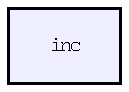
\includegraphics[width=49pt]{dir_ef15eccf5bd9eca446a41a18c57ac0fd_dep}
\end{center}
\end{figure}
\subsection*{Files}
\begin{CompactItemize}
\item 
file \textbf{Classifier.hpp}
\item 
file \hyperlink{_clip_8hpp}{Clip.hpp}
\begin{CompactList}\small\item\em Declaration of the class \hyperlink{class_clip}{Clip}. \item\end{CompactList}

\item 
file \hyperlink{_clip_location_8hpp}{ClipLocation.hpp}
\begin{CompactList}\small\item\em Declaration of the class \hyperlink{class_clip_location}{ClipLocation}. \item\end{CompactList}

\item 
file \textbf{FeatureVector.hpp}
\item 
file \hyperlink{_nessie_exception_8hpp}{NessieException.hpp}
\begin{CompactList}\small\item\em Declaration of the class \hyperlink{class_nessie_exception}{NessieException}. \item\end{CompactList}

\item 
file \hyperlink{_pixel_8hpp}{Pixel.hpp}
\begin{CompactList}\small\item\em Declaration of the custom type Pixel. \item\end{CompactList}

\item 
file \hyperlink{_preprocessor_8hpp}{Preprocessor.hpp}
\begin{CompactList}\small\item\em Declaration of the class \hyperlink{class_preprocessor}{Preprocessor}. \item\end{CompactList}

\item 
file \hyperlink{_recognizer_8hpp}{Recognizer.hpp}
\begin{CompactList}\small\item\em Declaration of the class \hyperlink{class_recognizer}{Recognizer}. \item\end{CompactList}

\item 
file \hyperlink{_segmenter_8hpp}{Segmenter.hpp}
\begin{CompactList}\small\item\em Declaration of the class \hyperlink{class_segmenter}{Segmenter}. \item\end{CompactList}

\item 
file \hyperlink{_shape_8hpp}{Shape.hpp}
\begin{CompactList}\small\item\em Declaration of the class \hyperlink{class_shape}{Shape}. \item\end{CompactList}

\item 
file \hyperlink{_statistics_8hpp}{Statistics.hpp}
\begin{CompactList}\small\item\em Declaration of the class \hyperlink{class_statistics}{Statistics}. \item\end{CompactList}

\item 
file \hyperlink{_text_8hpp}{Text.hpp}
\begin{CompactList}\small\item\em Declaration of the class \hyperlink{class_text}{Text}. \item\end{CompactList}

\end{CompactItemize}

\hypertarget{dir_f108b8e716a38a781a23bf0e62a4b450}{
\section{src/ Directory Reference}
\label{dir_f108b8e716a38a781a23bf0e62a4b450}\index{src/ Directory Reference@{src/ Directory Reference}}
}




\nopagebreak
\begin{figure}[H]
\begin{center}
\leavevmode
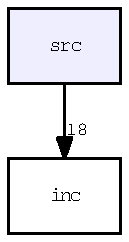
\includegraphics[width=49pt]{dir_f108b8e716a38a781a23bf0e62a4b450_dep}
\end{center}
\end{figure}
\subsection*{Files}
\begin{CompactItemize}
\item 
file \textbf{Classifier.cpp}
\item 
file \hyperlink{_clip_8cpp}{Clip.cpp}
\begin{CompactList}\small\item\em Implementation of the class \hyperlink{class_clip}{Clip}. \item\end{CompactList}

\item 
file \hyperlink{_clip_location_8cpp}{ClipLocation.cpp}
\begin{CompactList}\small\item\em Implementation of the class \hyperlink{class_clip_location}{ClipLocation}. \item\end{CompactList}

\item 
file \textbf{FeatureVector.cpp}
\item 
file \hyperlink{main_8cpp}{main.cpp}
\begin{CompactList}\small\item\em Implementation of a command line program for testing purposes. \item\end{CompactList}

\item 
file \hyperlink{_nessie_exception_8cpp}{NessieException.cpp}
\begin{CompactList}\small\item\em Implementation of the class \hyperlink{class_nessie_exception}{NessieException}. \item\end{CompactList}

\item 
file \hyperlink{_preprocessor_8cpp}{Preprocessor.cpp}
\begin{CompactList}\small\item\em Implementation of the class \hyperlink{class_preprocessor}{Preprocessor}. \item\end{CompactList}

\item 
file \hyperlink{_recognizer_8cpp}{Recognizer.cpp}
\begin{CompactList}\small\item\em Implementation of the class \hyperlink{class_recognizer}{Recognizer}. \item\end{CompactList}

\item 
file \hyperlink{_segmenter_8cpp}{Segmenter.cpp}
\begin{CompactList}\small\item\em Definition of the class \hyperlink{class_segmenter}{Segmenter}. \item\end{CompactList}

\item 
file \hyperlink{_shape_8cpp}{Shape.cpp}
\begin{CompactList}\small\item\em Implementation of the class \hyperlink{class_shape}{Shape}. \item\end{CompactList}

\item 
file \hyperlink{_statistics_8cpp}{Statistics.cpp}
\begin{CompactList}\small\item\em Implementation of the class \hyperlink{class_statistics}{Statistics}. \item\end{CompactList}

\item 
file \hyperlink{_text_8cpp}{Text.cpp}
\begin{CompactList}\small\item\em Implementation of the class \hyperlink{class_text}{Text}. \item\end{CompactList}

\end{CompactItemize}

\chapter{Data Structure Documentation}
\hypertarget{struct_font_color}{
\section{FontColor Struct Reference}
\label{struct_font_color}\index{FontColor@{FontColor}}
}
{\tt \#include $<$FontColor.h$>$}



\subsection{Detailed Description}
Font color of a character. 

This struct represents the color of font that a character has. The color value is stored using the RGB color space with 256 values per component, and the three components separated.

\begin{Desc}
\item[Author:]Eliezer Talón (\href{mailto:elitalon@gmail.com}{\tt elitalon@gmail.com}) \end{Desc}
\begin{Desc}
\item[Date:]2008-09-18 \end{Desc}


Definition at line 14 of file FontColor.h.\subsection*{Public Member Functions}
\begin{CompactItemize}
\item 
\hyperlink{struct_font_color_c96e70b5ab153ea18d1e3196f79da1ab}{FontColor} ()
\begin{CompactList}\small\item\em Constructor. \item\end{CompactList}\item 
\hyperlink{struct_font_color_7ed65a063287bfa5ba792bd4d85c1b51}{FontColor} (unsigned int red\_\-, unsigned int green\_\-, unsigned int blue\_\-)
\begin{CompactList}\small\item\em Constructor. \item\end{CompactList}\item 
\hyperlink{struct_font_color_660917a7d04fdf47910573165f67cdaa}{$\sim$FontColor} ()
\begin{CompactList}\small\item\em Destructor. \item\end{CompactList}\end{CompactItemize}
\subsection*{Data Fields}
\begin{CompactItemize}
\item 
\hypertarget{struct_font_color_c8239f8b8a384f8aea88b5c722bca5d3}{
unsigned int \hyperlink{struct_font_color_c8239f8b8a384f8aea88b5c722bca5d3}{red}}
\label{struct_font_color_c8239f8b8a384f8aea88b5c722bca5d3}

\begin{CompactList}\small\item\em Red component. \item\end{CompactList}\item 
\hypertarget{struct_font_color_a44da3bcb5ab54c9e353795e2b665845}{
unsigned int \hyperlink{struct_font_color_a44da3bcb5ab54c9e353795e2b665845}{green}}
\label{struct_font_color_a44da3bcb5ab54c9e353795e2b665845}

\begin{CompactList}\small\item\em Green component. \item\end{CompactList}\item 
\hypertarget{struct_font_color_82808b069e5c057f443aa2eddb6f5b71}{
unsigned int \hyperlink{struct_font_color_82808b069e5c057f443aa2eddb6f5b71}{blue}}
\label{struct_font_color_82808b069e5c057f443aa2eddb6f5b71}

\begin{CompactList}\small\item\em Blue component. \item\end{CompactList}\end{CompactItemize}


\subsection{Constructor \& Destructor Documentation}
\hypertarget{struct_font_color_c96e70b5ab153ea18d1e3196f79da1ab}{
\index{FontColor@{FontColor}!FontColor@{FontColor}}
\index{FontColor@{FontColor}!FontColor@{FontColor}}
\subsubsection[FontColor]{\setlength{\rightskip}{0pt plus 5cm}FontColor::FontColor ()}}
\label{struct_font_color_c96e70b5ab153ea18d1e3196f79da1ab}


Constructor. 

Initializes a \hyperlink{struct_font_color}{FontColor} object with all RGB components set to 0

\begin{Desc}
\item[Author:]Eliezer Talón (\href{mailto:elitalon@gmail.com}{\tt elitalon@gmail.com}) \end{Desc}
\begin{Desc}
\item[Date:]2008-09-18 \end{Desc}


Definition at line 10 of file FontColor.cpp.\hypertarget{struct_font_color_7ed65a063287bfa5ba792bd4d85c1b51}{
\index{FontColor@{FontColor}!FontColor@{FontColor}}
\index{FontColor@{FontColor}!FontColor@{FontColor}}
\subsubsection[FontColor]{\setlength{\rightskip}{0pt plus 5cm}FontColor::FontColor (unsigned int {\em red\_\-}, \/  unsigned int {\em green\_\-}, \/  unsigned int {\em blue\_\-})}}
\label{struct_font_color_7ed65a063287bfa5ba792bd4d85c1b51}


Constructor. 

Initializes a \hyperlink{struct_font_color}{FontColor} object with the components set to the values passed. Since the color must be expressed using a RGB scale of 256 possible values, any value over 255 will be truncated

\begin{Desc}
\item[Author:]Eliezer Talón (\href{mailto:elitalon@gmail.com}{\tt elitalon@gmail.com}) \end{Desc}
\begin{Desc}
\item[Date:]2008-09-18 \end{Desc}


Definition at line 24 of file FontColor.cpp.\hypertarget{struct_font_color_660917a7d04fdf47910573165f67cdaa}{
\index{FontColor@{FontColor}!$\sim$FontColor@{$\sim$FontColor}}
\index{$\sim$FontColor@{$\sim$FontColor}!FontColor@{FontColor}}
\subsubsection[$\sim$FontColor]{\setlength{\rightskip}{0pt plus 5cm}FontColor::$\sim$FontColor ()}}
\label{struct_font_color_660917a7d04fdf47910573165f67cdaa}


Destructor. 

Destroys a \hyperlink{struct_font_color}{FontColor} object

\begin{Desc}
\item[Author:]Eliezer Talón (\href{mailto:elitalon@gmail.com}{\tt elitalon@gmail.com}) \end{Desc}
\begin{Desc}
\item[Date:]2008-09-18 \end{Desc}


Definition at line 37 of file FontColor.cpp.

The documentation for this struct was generated from the following files:\begin{CompactItemize}
\item 
FontColor.h (110)\item 
FontColor.cpp (111)\end{CompactItemize}

\hypertarget{struct_statistics}{
\section{Statistics Struct Reference}
\label{struct_statistics}\index{Statistics@{Statistics}}
}
{\tt \#include $<$Statistics.h$>$}



\subsection{Detailed Description}
\hyperlink{struct_statistics}{Statistics} about a text and its recognition process. 

This struct stores a number of statistic data regarding the recognition process and the text produced.

First, it stores the elapsed time on every stage, accumulated internally in the critical processes (mostly, image processing algorithms). Second, it also stores the number of words in the text and the appearance rate of every single word.

\begin{Desc}
\item[Author:]Eliezer Talón (\href{mailto:elitalon@gmail.com}{\tt elitalon@gmail.com}) \end{Desc}
\begin{Desc}
\item[Date:]2008-09-18 \end{Desc}


Definition at line 24 of file Statistics.h.\subsection*{Public Member Functions}
\begin{CompactItemize}
\item 
\hyperlink{struct_statistics_60ddd90a571ed4c3ce8c0f6317a36d63}{Statistics} ()
\begin{CompactList}\small\item\em Constructor. \item\end{CompactList}\item 
\hyperlink{struct_statistics_b68ede75479e44d5c35b78ec1284065b}{$\sim$Statistics} ()
\begin{CompactList}\small\item\em Destructor. \item\end{CompactList}\end{CompactItemize}
\subsection*{Data Fields}
\begin{CompactItemize}
\item 
\hypertarget{struct_statistics_b8aec77e19e962544468c569a8333d15}{
unsigned int \hyperlink{struct_statistics_b8aec77e19e962544468c569a8333d15}{nWords}}
\label{struct_statistics_b8aec77e19e962544468c569a8333d15}

\begin{CompactList}\small\item\em Number of words in the recognized text. \item\end{CompactList}\item 
\hypertarget{struct_statistics_905896f578b6af9e46d82990e39480bd}{
vector$<$ \hyperlink{_word_rate_8h_e8f43926daba5798edbb3cb94ad07ff7}{WordRate} $>$ \hyperlink{struct_statistics_905896f578b6af9e46d82990e39480bd}{wordRates}}
\label{struct_statistics_905896f578b6af9e46d82990e39480bd}

\begin{CompactList}\small\item\em List of appearance rates of every word in the recognized text. \item\end{CompactList}\item 
\hypertarget{struct_statistics_4a194feb4de2fc619d311b2adb2a7e74}{
double \hyperlink{struct_statistics_4a194feb4de2fc619d311b2adb2a7e74}{noiseRemovalTime}}
\label{struct_statistics_4a194feb4de2fc619d311b2adb2a7e74}

\begin{CompactList}\small\item\em Elapsed time in the noise removal stage. \item\end{CompactList}\item 
\hypertarget{struct_statistics_fc22ca2705714cfc44c45c772475c1cb}{
double \hyperlink{struct_statistics_fc22ca2705714cfc44c45c772475c1cb}{grayscaleConversionTime}}
\label{struct_statistics_fc22ca2705714cfc44c45c772475c1cb}

\begin{CompactList}\small\item\em Elapsed time in the grayscale conversion stage. \item\end{CompactList}\item 
\hypertarget{struct_statistics_6c2cd48482d1de181cb2dd32b3315449}{
double \hyperlink{struct_statistics_6c2cd48482d1de181cb2dd32b3315449}{floodFillingTime}}
\label{struct_statistics_6c2cd48482d1de181cb2dd32b3315449}

\begin{CompactList}\small\item\em Elapsed time in the flood filling stage. \item\end{CompactList}\item 
\hypertarget{struct_statistics_e2c88c8b599b217ad3f316cca7a15a23}{
double \hyperlink{struct_statistics_e2c88c8b599b217ad3f316cca7a15a23}{thresholdingTime}}
\label{struct_statistics_e2c88c8b599b217ad3f316cca7a15a23}

\begin{CompactList}\small\item\em Elapsed time in the thresholding stage. \item\end{CompactList}\item 
\hypertarget{struct_statistics_ae46d5f7b2a374dd79b15533facc9e6c}{
double \hyperlink{struct_statistics_ae46d5f7b2a374dd79b15533facc9e6c}{featureVectorsBuildingTime}}
\label{struct_statistics_ae46d5f7b2a374dd79b15533facc9e6c}

\begin{CompactList}\small\item\em Elapsed time in the feature vectors building stage. \item\end{CompactList}\item 
\hypertarget{struct_statistics_1e09de36cf3a65ab2a471e877578257d}{
double \hyperlink{struct_statistics_1e09de36cf3a65ab2a471e877578257d}{charactersExtractionTime}}
\label{struct_statistics_1e09de36cf3a65ab2a471e877578257d}

\begin{CompactList}\small\item\em Elapsed time in the characters extraction stage. \item\end{CompactList}\item 
\hypertarget{struct_statistics_7bfcefbca86812a13371f35f6ad2632c}{
double \hyperlink{struct_statistics_7bfcefbca86812a13371f35f6ad2632c}{classificationTime}}
\label{struct_statistics_7bfcefbca86812a13371f35f6ad2632c}

\begin{CompactList}\small\item\em Returns the total time within the classification stage. \item\end{CompactList}\item 
\hypertarget{struct_statistics_f5afa8bf14678df2d5b869b6161a209f}{
double \hyperlink{struct_statistics_f5afa8bf14678df2d5b869b6161a209f}{segmentationTime}}
\label{struct_statistics_f5afa8bf14678df2d5b869b6161a209f}

\begin{CompactList}\small\item\em Returns the total time within the segmentation stage. \item\end{CompactList}\item 
\hypertarget{struct_statistics_57aa8970c666c415db6dcdd0cc3920f6}{
double \hyperlink{struct_statistics_57aa8970c666c415db6dcdd0cc3920f6}{preprocessingTime}}
\label{struct_statistics_57aa8970c666c415db6dcdd0cc3920f6}

\begin{CompactList}\small\item\em Returns the total time within the preprocessing stage. \item\end{CompactList}\end{CompactItemize}


\subsection{Constructor \& Destructor Documentation}
\hypertarget{struct_statistics_60ddd90a571ed4c3ce8c0f6317a36d63}{
\index{Statistics@{Statistics}!Statistics@{Statistics}}
\index{Statistics@{Statistics}!Statistics@{Statistics}}
\subsubsection[Statistics]{\setlength{\rightskip}{0pt plus 5cm}Statistics::Statistics ()}}
\label{struct_statistics_60ddd90a571ed4c3ce8c0f6317a36d63}


Constructor. 

Initializes a \hyperlink{struct_statistics}{Statistics} object with timers set to 0

\begin{Desc}
\item[Author:]Eliezer Talón (\href{mailto:elitalon@gmail.com}{\tt elitalon@gmail.com}) \end{Desc}
\begin{Desc}
\item[Date:]2008-09-22 \end{Desc}


Definition at line 10 of file Statistics.cpp.\hypertarget{struct_statistics_b68ede75479e44d5c35b78ec1284065b}{
\index{Statistics@{Statistics}!$\sim$Statistics@{$\sim$Statistics}}
\index{$\sim$Statistics@{$\sim$Statistics}!Statistics@{Statistics}}
\subsubsection[$\sim$Statistics]{\setlength{\rightskip}{0pt plus 5cm}Statistics::$\sim$Statistics ()}}
\label{struct_statistics_b68ede75479e44d5c35b78ec1284065b}


Destructor. 

Destroys a \hyperlink{struct_statistics}{Statistics} object

\begin{Desc}
\item[Author:]Eliezer Talón (\href{mailto:elitalon@gmail.com}{\tt elitalon@gmail.com}) \end{Desc}
\begin{Desc}
\item[Date:]2008-09-17 \end{Desc}


Definition at line 25 of file Statistics.cpp.

The documentation for this struct was generated from the following files:\begin{CompactItemize}
\item 
Statistics.h (111)\item 
Statistics.cpp (111)\end{CompactItemize}

\hypertarget{class_style}{
\section{Style Class Reference}
\label{class_style}\index{Style@{Style}}
}
{\tt \#include $<$Style.h$>$}

Collaboration diagram for Style:\nopagebreak
\begin{figure}[H]
\begin{center}
\leavevmode
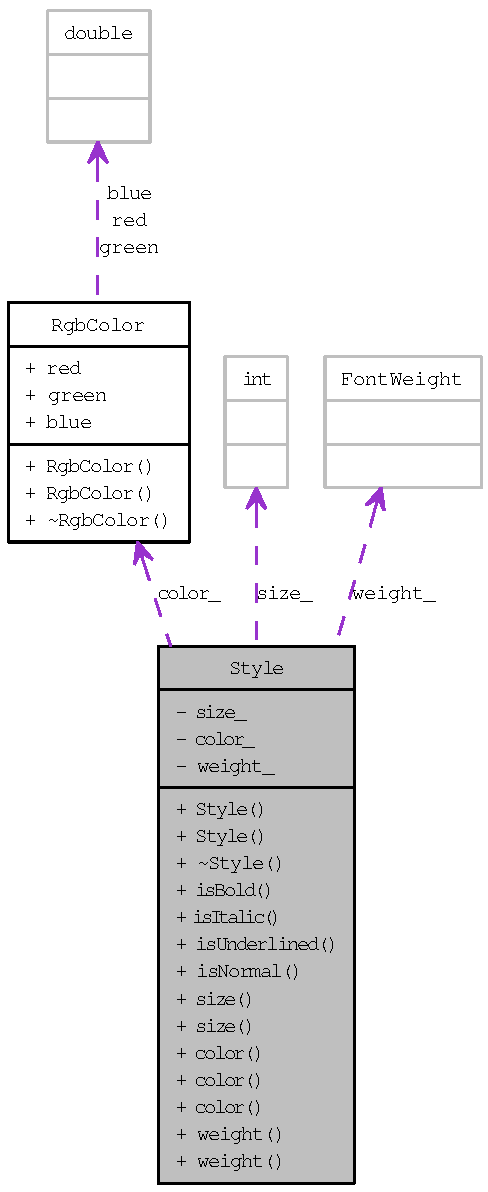
\includegraphics[height=400pt]{class_style__coll__graph}
\end{center}
\end{figure}


\subsection{Detailed Description}
Font style of a character. 

This class stores information about the font style of a character in the recognized text. Due to the different design styles in newspapers, a text may contain different kinds of style. That's why we must keep the style of every single character.

\begin{Desc}
\item[Author:]Eliezer Talón (\href{mailto:elitalon@gmail.com}{\tt elitalon@gmail.com}) \end{Desc}
\begin{Desc}
\item[Date:]2008-09-25 \end{Desc}


Definition at line 24 of file Style.h.\subsection*{Public Member Functions}
\begin{CompactItemize}
\item 
\hyperlink{class_style_914f187818eb30c0cebe3df5378bfa0a}{Style} ()
\begin{CompactList}\small\item\em Constructor. \item\end{CompactList}\item 
\hyperlink{class_style_69801b8ce2b1520ef24e1a84d04609e5}{Style} (unsigned int size, \hyperlink{struct_rgb_color}{RgbColor} color, \hyperlink{_font_weight_8h_ecff23ba4a68486421bcea57e095fe66}{FontWeight} weight)
\begin{CompactList}\small\item\em Constructor. \item\end{CompactList}\item 
\hyperlink{class_style_7c798ef9b77bc94719542feade497725}{$\sim$Style} ()
\begin{CompactList}\small\item\em Destructor. \item\end{CompactList}\item 
bool \hyperlink{class_style_59d23709575c5e6e5434ef0af5ff94b6}{isBold} () const 
\begin{CompactList}\small\item\em Returns true if the font weight is bold. \item\end{CompactList}\item 
bool \hyperlink{class_style_5d57a686b93123e8ca5f8f91afb596c1}{isItalic} () const 
\begin{CompactList}\small\item\em Returns true if the font weight is italic. \item\end{CompactList}\item 
bool \hyperlink{class_style_d1fcc32d8b565aae007012eb603fedcd}{isUnderlined} () const 
\begin{CompactList}\small\item\em Returns true if the font weight is underlined. \item\end{CompactList}\item 
bool \hyperlink{class_style_db2cbc7ca50b2f5c632c8e9b0420044c}{isNormal} () const 
\begin{CompactList}\small\item\em Returns true if the font weight is normal. \item\end{CompactList}\item 
unsigned int \hyperlink{class_style_9356c4a5d30f4e0f5c86f8c8b3f36cd2}{getSize} () const 
\begin{CompactList}\small\item\em Returns the font size. \item\end{CompactList}\item 
void \hyperlink{class_style_1338ebe3d562a710fdc26f49d0082a7c}{setSize} (unsigned int size)
\begin{CompactList}\small\item\em Sets the font size. \item\end{CompactList}\item 
\hyperlink{struct_rgb_color}{RgbColor} \hyperlink{class_style_bd212fb31bc7e1e7502c18f9e0b6734c}{getColor} () const 
\begin{CompactList}\small\item\em Returns the font color. \item\end{CompactList}\item 
void \hyperlink{class_style_596534e321ac5c2f4444192f2cc0d793}{setColor} (\hyperlink{struct_rgb_color}{RgbColor} color)
\begin{CompactList}\small\item\em Sets the font color. \item\end{CompactList}\item 
void \hyperlink{class_style_8162fb5c89458b1892f1802231a63a16}{setColor} (double red, double green, double blue)
\begin{CompactList}\small\item\em Sets the font color. \item\end{CompactList}\item 
\hyperlink{_font_weight_8h_ecff23ba4a68486421bcea57e095fe66}{FontWeight} \hyperlink{class_style_5798e7a57bb2df5e37aa0cdc5606a8b3}{getWeight} () const 
\begin{CompactList}\small\item\em Returns the font weight. \item\end{CompactList}\item 
void \hyperlink{class_style_3bb5ced743176c5a68479d506f348350}{setWeight} (\hyperlink{_font_weight_8h_ecff23ba4a68486421bcea57e095fe66}{FontWeight} weight)
\begin{CompactList}\small\item\em Sets the font weight. \item\end{CompactList}\end{CompactItemize}
\subsection*{Private Attributes}
\begin{CompactItemize}
\item 
\hypertarget{class_style_25ff6a0bb75d86d204711507f8d8865e}{
unsigned int \hyperlink{class_style_25ff6a0bb75d86d204711507f8d8865e}{size\_\-}}
\label{class_style_25ff6a0bb75d86d204711507f8d8865e}

\begin{CompactList}\small\item\em Size of the character in points. \item\end{CompactList}\item 
\hypertarget{class_style_cfd308751180d820aac54f5d96951f34}{
\hyperlink{struct_rgb_color}{RgbColor} \hyperlink{class_style_cfd308751180d820aac54f5d96951f34}{color\_\-}}
\label{class_style_cfd308751180d820aac54f5d96951f34}

\begin{CompactList}\small\item\em Color of the character. \item\end{CompactList}\item 
\hypertarget{class_style_82e4a1ebf54db6abc6fa3e23706a6aa8}{
\hyperlink{_font_weight_8h_ecff23ba4a68486421bcea57e095fe66}{FontWeight} \hyperlink{class_style_82e4a1ebf54db6abc6fa3e23706a6aa8}{weight\_\-}}
\label{class_style_82e4a1ebf54db6abc6fa3e23706a6aa8}

\begin{CompactList}\small\item\em Font weight of the character. \item\end{CompactList}\end{CompactItemize}


\subsection{Constructor \& Destructor Documentation}
\hypertarget{class_style_914f187818eb30c0cebe3df5378bfa0a}{
\index{Style@{Style}!Style@{Style}}
\index{Style@{Style}!Style@{Style}}
\subsubsection[Style]{\setlength{\rightskip}{0pt plus 5cm}Style::Style ()}}
\label{class_style_914f187818eb30c0cebe3df5378bfa0a}


Constructor. 

Initializes a \hyperlink{class_style}{Style} object with size set to 0, color set to black and weight set to normal

\begin{Desc}
\item[Author:]Eliezer Talón (\href{mailto:elitalon@gmail.com}{\tt elitalon@gmail.com}) \end{Desc}
\begin{Desc}
\item[Date:]2008-09-25 \end{Desc}


Definition at line 15 of file Style.cpp.\hypertarget{class_style_69801b8ce2b1520ef24e1a84d04609e5}{
\index{Style@{Style}!Style@{Style}}
\index{Style@{Style}!Style@{Style}}
\subsubsection[Style]{\setlength{\rightskip}{0pt plus 5cm}Style::Style (unsigned int {\em size}, \/  {\bf RgbColor} {\em color}, \/  {\bf FontWeight} {\em weight})}}
\label{class_style_69801b8ce2b1520ef24e1a84d04609e5}


Constructor. 

Initializes a \hyperlink{class_style}{Style} object with size, color and weight set to the values passed

\begin{Desc}
\item[Author:]Eliezer Talón (\href{mailto:elitalon@gmail.com}{\tt elitalon@gmail.com}) \end{Desc}
\begin{Desc}
\item[Date:]2008-09-25 \end{Desc}


Definition at line 27 of file Style.cpp.\hypertarget{class_style_7c798ef9b77bc94719542feade497725}{
\index{Style@{Style}!$\sim$Style@{$\sim$Style}}
\index{$\sim$Style@{$\sim$Style}!Style@{Style}}
\subsubsection[$\sim$Style]{\setlength{\rightskip}{0pt plus 5cm}Style::$\sim$Style ()}}
\label{class_style_7c798ef9b77bc94719542feade497725}


Destructor. 

Destroys a \hyperlink{class_style}{Style} object

\begin{Desc}
\item[Author:]Eliezer Talón (\href{mailto:elitalon@gmail.com}{\tt elitalon@gmail.com}) \end{Desc}
\begin{Desc}
\item[Date:]2008-09-23 \end{Desc}


Definition at line 39 of file Style.cpp.

\subsection{Member Function Documentation}
\hypertarget{class_style_59d23709575c5e6e5434ef0af5ff94b6}{
\index{Style@{Style}!isBold@{isBold}}
\index{isBold@{isBold}!Style@{Style}}
\subsubsection[isBold]{\setlength{\rightskip}{0pt plus 5cm}bool Style::isBold () const}}
\label{class_style_59d23709575c5e6e5434ef0af5ff94b6}


Returns true if the font weight is bold. 

A bold font may be only bold, bold and italic or bold and underlined

\begin{Desc}
\item[Author:]Eliezer Talón (\href{mailto:elitalon@gmail.com}{\tt elitalon@gmail.com}) \end{Desc}
\begin{Desc}
\item[Date:]2008-09-23 \end{Desc}


Definition at line 51 of file Style.cpp.\hypertarget{class_style_5d57a686b93123e8ca5f8f91afb596c1}{
\index{Style@{Style}!isItalic@{isItalic}}
\index{isItalic@{isItalic}!Style@{Style}}
\subsubsection[isItalic]{\setlength{\rightskip}{0pt plus 5cm}bool Style::isItalic () const}}
\label{class_style_5d57a686b93123e8ca5f8f91afb596c1}


Returns true if the font weight is italic. 

An italic font may be only italic, italic and bold or italic and underlined

\begin{Desc}
\item[Author:]Eliezer Talón (\href{mailto:elitalon@gmail.com}{\tt elitalon@gmail.com}) \end{Desc}
\begin{Desc}
\item[Date:]2008-09-23 \end{Desc}


Definition at line 75 of file Style.cpp.\hypertarget{class_style_d1fcc32d8b565aae007012eb603fedcd}{
\index{Style@{Style}!isUnderlined@{isUnderlined}}
\index{isUnderlined@{isUnderlined}!Style@{Style}}
\subsubsection[isUnderlined]{\setlength{\rightskip}{0pt plus 5cm}bool Style::isUnderlined () const}}
\label{class_style_d1fcc32d8b565aae007012eb603fedcd}


Returns true if the font weight is underlined. 

An underlined font may be only underlined, underlined and italic or underlined and bold

\begin{Desc}
\item[Author:]Eliezer Talón (\href{mailto:elitalon@gmail.com}{\tt elitalon@gmail.com}) \end{Desc}
\begin{Desc}
\item[Date:]2008-09-23 \end{Desc}


Definition at line 99 of file Style.cpp.\hypertarget{class_style_db2cbc7ca50b2f5c632c8e9b0420044c}{
\index{Style@{Style}!isNormal@{isNormal}}
\index{isNormal@{isNormal}!Style@{Style}}
\subsubsection[isNormal]{\setlength{\rightskip}{0pt plus 5cm}bool Style::isNormal () const}}
\label{class_style_db2cbc7ca50b2f5c632c8e9b0420044c}


Returns true if the font weight is normal. 

A normal font is neither bold, nor italic, nor underlined

\begin{Desc}
\item[Author:]Eliezer Talón (\href{mailto:elitalon@gmail.com}{\tt elitalon@gmail.com}) \end{Desc}
\begin{Desc}
\item[Date:]2008-09-23 \end{Desc}


Definition at line 123 of file Style.cpp.\hypertarget{class_style_9356c4a5d30f4e0f5c86f8c8b3f36cd2}{
\index{Style@{Style}!getSize@{getSize}}
\index{getSize@{getSize}!Style@{Style}}
\subsubsection[getSize]{\setlength{\rightskip}{0pt plus 5cm}unsigned int Style::getSize () const}}
\label{class_style_9356c4a5d30f4e0f5c86f8c8b3f36cd2}


Returns the font size. 

The size is expressed in points (pt)

\begin{Desc}
\item[Author:]Eliezer Talón (\href{mailto:elitalon@gmail.com}{\tt elitalon@gmail.com}) \end{Desc}
\begin{Desc}
\item[Date:]2008-09-23 \end{Desc}


Definition at line 147 of file Style.cpp.\hypertarget{class_style_1338ebe3d562a710fdc26f49d0082a7c}{
\index{Style@{Style}!setSize@{setSize}}
\index{setSize@{setSize}!Style@{Style}}
\subsubsection[setSize]{\setlength{\rightskip}{0pt plus 5cm}void Style::setSize (unsigned int {\em size})}}
\label{class_style_1338ebe3d562a710fdc26f49d0082a7c}


Sets the font size. 

The size is expressed in points (pt)

\begin{Desc}
\item[Author:]Eliezer Talón (\href{mailto:elitalon@gmail.com}{\tt elitalon@gmail.com}) \end{Desc}
\begin{Desc}
\item[Date:]2008-09-23 \end{Desc}


Definition at line 159 of file Style.cpp.\hypertarget{class_style_bd212fb31bc7e1e7502c18f9e0b6734c}{
\index{Style@{Style}!getColor@{getColor}}
\index{getColor@{getColor}!Style@{Style}}
\subsubsection[getColor]{\setlength{\rightskip}{0pt plus 5cm}{\bf RgbColor} Style::getColor () const}}
\label{class_style_bd212fb31bc7e1e7502c18f9e0b6734c}


Returns the font color. 

\begin{Desc}
\item[See also:]\hyperlink{struct_rgb_color}{RgbColor}\end{Desc}
\begin{Desc}
\item[Author:]Eliezer Talón (\href{mailto:elitalon@gmail.com}{\tt elitalon@gmail.com}) \end{Desc}
\begin{Desc}
\item[Date:]2008-09-25 \end{Desc}


Definition at line 171 of file Style.cpp.\hypertarget{class_style_596534e321ac5c2f4444192f2cc0d793}{
\index{Style@{Style}!setColor@{setColor}}
\index{setColor@{setColor}!Style@{Style}}
\subsubsection[setColor]{\setlength{\rightskip}{0pt plus 5cm}void Style::setColor ({\bf RgbColor} {\em color})}}
\label{class_style_596534e321ac5c2f4444192f2cc0d793}


Sets the font color. 

\begin{Desc}
\item[See also:]\hyperlink{struct_rgb_color}{RgbColor}\end{Desc}
\begin{Desc}
\item[Author:]Eliezer Talón (\href{mailto:elitalon@gmail.com}{\tt elitalon@gmail.com}) \end{Desc}
\begin{Desc}
\item[Date:]2008-09-25 \end{Desc}


Definition at line 183 of file Style.cpp.\hypertarget{class_style_8162fb5c89458b1892f1802231a63a16}{
\index{Style@{Style}!setColor@{setColor}}
\index{setColor@{setColor}!Style@{Style}}
\subsubsection[setColor]{\setlength{\rightskip}{0pt plus 5cm}void Style::setColor (double {\em red}, \/  double {\em green}, \/  double {\em blue})}}
\label{class_style_8162fb5c89458b1892f1802231a63a16}


Sets the font color. 

The font color is created internally as a \hyperlink{struct_rgb_color}{RgbColor} object with the values passed

\begin{Desc}
\item[See also:]\hyperlink{struct_rgb_color}{RgbColor}\end{Desc}
\begin{Desc}
\item[Author:]Eliezer Talón (\href{mailto:elitalon@gmail.com}{\tt elitalon@gmail.com}) \end{Desc}
\begin{Desc}
\item[Date:]2008-09-25 \end{Desc}


Definition at line 197 of file Style.cpp.\hypertarget{class_style_5798e7a57bb2df5e37aa0cdc5606a8b3}{
\index{Style@{Style}!getWeight@{getWeight}}
\index{getWeight@{getWeight}!Style@{Style}}
\subsubsection[getWeight]{\setlength{\rightskip}{0pt plus 5cm}{\bf FontWeight} Style::getWeight () const}}
\label{class_style_5798e7a57bb2df5e37aa0cdc5606a8b3}


Returns the font weight. 

\begin{Desc}
\item[See also:]\hyperlink{_font_weight_8h_ecff23ba4a68486421bcea57e095fe66}{FontWeight}\end{Desc}
\begin{Desc}
\item[Author:]Eliezer Talón (\href{mailto:elitalon@gmail.com}{\tt elitalon@gmail.com}) \end{Desc}
\begin{Desc}
\item[Date:]2008-09-23 \end{Desc}


Definition at line 209 of file Style.cpp.\hypertarget{class_style_3bb5ced743176c5a68479d506f348350}{
\index{Style@{Style}!setWeight@{setWeight}}
\index{setWeight@{setWeight}!Style@{Style}}
\subsubsection[setWeight]{\setlength{\rightskip}{0pt plus 5cm}void Style::setWeight ({\bf FontWeight} {\em weight})}}
\label{class_style_3bb5ced743176c5a68479d506f348350}


Sets the font weight. 

The weight must be passed using a literal value of FontWeight enumeration.

\begin{Desc}
\item[See also:]\hyperlink{_font_weight_8h_ecff23ba4a68486421bcea57e095fe66}{FontWeight}\end{Desc}
\begin{Desc}
\item[Author:]Eliezer Talón (\href{mailto:elitalon@gmail.com}{\tt elitalon@gmail.com}) \end{Desc}
\begin{Desc}
\item[Date:]2008-09-23 \end{Desc}


Definition at line 223 of file Style.cpp.

The documentation for this class was generated from the following files:\begin{CompactItemize}
\item 
\hyperlink{_style_8h}{Style.h (111)}\item 
\hyperlink{_style_8cpp}{Style.cpp (111)}\end{CompactItemize}

\hypertarget{class_text}{
\section{Text Class Reference}
\label{class_text}\index{Text@{Text}}
}
{\tt \#include $<$Text.h$>$}

Collaboration diagram for Text:\nopagebreak
\begin{figure}[H]
\begin{center}
\leavevmode
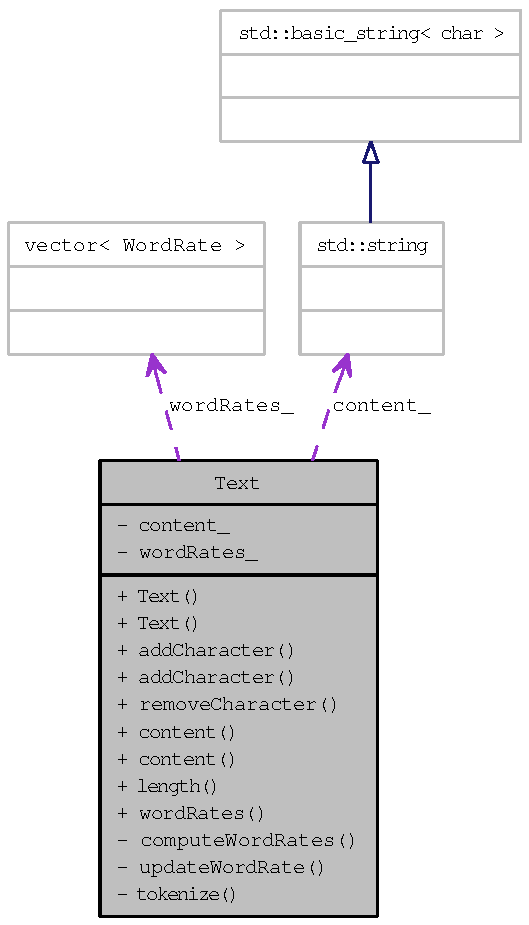
\includegraphics[height=400pt]{class_text__coll__graph}
\end{center}
\end{figure}


\subsection{Detailed Description}
\hyperlink{class_text}{Text} extracted by the recognizer. 

This class stores the text that has been extracted from the press clip during the recognition process. It also keeps the appearance rate of every word in text.

\begin{Desc}
\item[Author:]Eliezer Talón (\href{mailto:elitalon@gmail.com}{\tt elitalon@gmail.com}) \end{Desc}
\begin{Desc}
\item[Date:]2008-10-04 \end{Desc}


Definition at line 25 of file Text.h.\subsection*{Public Member Functions}
\begin{CompactItemize}
\item 
\hyperlink{class_text_b3e26143fccc52699bcc5149cae852bc}{Text} ()
\begin{CompactList}\small\item\em Constructor. \item\end{CompactList}\item 
\hyperlink{class_text_d8c7b52db022f4351e31b2b7609a8180}{Text} (const std::string \&content)
\begin{CompactList}\small\item\em Constructor. \item\end{CompactList}\item 
\hyperlink{class_text_2d49e5c280e205125b149f7777ae30c7}{$\sim$Text} ()
\begin{CompactList}\small\item\em Destructor. \item\end{CompactList}\item 
void \hyperlink{class_text_6e6da63c90af68639adc7dd1336f6bf9}{addCharacter} (const char \&character)
\begin{CompactList}\small\item\em Adds a character to text. \item\end{CompactList}\item 
void \hyperlink{class_text_fdd11ad0c90ca483d4cff3d74a64da9e}{addCharacter} (const char \&character, const unsigned int \&position)
\begin{CompactList}\small\item\em Adds a character to text. \item\end{CompactList}\item 
void \hyperlink{class_text_e04500eeada2a4a3bb00554b32263c52}{removeCharacter} (const unsigned int \&position)
\begin{CompactList}\small\item\em Removes a character from text. \item\end{CompactList}\item 
std::string \hyperlink{class_text_58a34fa2cfd0c240a7517132017b6a83}{content} () const 
\begin{CompactList}\small\item\em Returns the text's content. \item\end{CompactList}\item 
void \hyperlink{class_text_eca454f28010b6b3e7bd0d771b8eaeb2}{content} (const std::string \&content)
\begin{CompactList}\small\item\em Sets the text's content. \item\end{CompactList}\item 
unsigned int \hyperlink{class_text_8d76db538f8617fb8880ba3e4ff3e6a5}{length} () const 
\begin{CompactList}\small\item\em Returns the text's length. \item\end{CompactList}\item 
std::vector$<$ \hyperlink{_word_rate_8h_8cfef8793106ac45a83059bd5573cbb3}{WordRate} $>$ \hyperlink{class_text_1387d9767b65f80355f1bdede26a0f7b}{wordRates} () const 
\begin{CompactList}\small\item\em Returns the appearance rates of every single word in text. \item\end{CompactList}\end{CompactItemize}
\subsection*{Private Member Functions}
\begin{CompactItemize}
\item 
void \hyperlink{class_text_8239e13039bcc1c713f66f1236693706}{computeWordRates} ()
\begin{CompactList}\small\item\em Builds the vector of appearance rates of every word. \item\end{CompactList}\item 
void \hyperlink{class_text_7466754bf64f0c22b291edb2bd14ba99}{updateWordRate} (const std::string \&word\_\-)
\begin{CompactList}\small\item\em Increases by one the number of appearances of a word. \item\end{CompactList}\item 
void \hyperlink{class_text_3fe3daa80386d15a275523b18bde7fd9}{tokenize} (std::vector$<$ std::string $>$ \&tokens\_\-, const std::string \&delimiters\_\-=\char`\"{} ,.$\backslash$n$\backslash$t:;!¡¿?\&/()=$\backslash$\char`\"{}'\char`\"{}) const 
\begin{CompactList}\small\item\em Extracts every word surrounded by a set of delimiters. \item\end{CompactList}\end{CompactItemize}
\subsection*{Private Attributes}
\begin{CompactItemize}
\item 
\hypertarget{class_text_8c5acddb86730d41099c87da7e386f6c}{
std::string \hyperlink{class_text_8c5acddb86730d41099c87da7e386f6c}{content\_\-}}
\label{class_text_8c5acddb86730d41099c87da7e386f6c}

\begin{CompactList}\small\item\em The text's content. \item\end{CompactList}\item 
\hypertarget{class_text_ee3a9a1486714df08c8e73ccb605e729}{
std::vector$<$ \hyperlink{_word_rate_8h_8cfef8793106ac45a83059bd5573cbb3}{WordRate} $>$ \hyperlink{class_text_ee3a9a1486714df08c8e73ccb605e729}{wordRates\_\-}}
\label{class_text_ee3a9a1486714df08c8e73ccb605e729}

\begin{CompactList}\small\item\em A list of appearance rates of every single word in text. \item\end{CompactList}\end{CompactItemize}


\subsection{Constructor \& Destructor Documentation}
\hypertarget{class_text_b3e26143fccc52699bcc5149cae852bc}{
\index{Text@{Text}!Text@{Text}}
\index{Text@{Text}!Text@{Text}}
\subsubsection[Text]{\setlength{\rightskip}{0pt plus 5cm}Text::Text ()}}
\label{class_text_b3e26143fccc52699bcc5149cae852bc}


Constructor. 

Initializes a \hyperlink{class_text}{Text} object with no content

\begin{Desc}
\item[Author:]Eliezer Talón (\href{mailto:elitalon@gmail.com}{\tt elitalon@gmail.com}) \end{Desc}
\begin{Desc}
\item[Date:]2008-10-04 \end{Desc}


Definition at line 19 of file Text.cpp.\hypertarget{class_text_d8c7b52db022f4351e31b2b7609a8180}{
\index{Text@{Text}!Text@{Text}}
\index{Text@{Text}!Text@{Text}}
\subsubsection[Text]{\setlength{\rightskip}{0pt plus 5cm}Text::Text (const std::string \& {\em content})}}
\label{class_text_d8c7b52db022f4351e31b2b7609a8180}


Constructor. 

Initializes a \hyperlink{class_text}{Text} object with the content passed

\begin{Desc}
\item[Parameters:]
\begin{description}
\item[{\em content}]Initial text\end{description}
\end{Desc}
\begin{Desc}
\item[Author:]Eliezer Talón (\href{mailto:elitalon@gmail.com}{\tt elitalon@gmail.com}) \end{Desc}
\begin{Desc}
\item[Date:]2008-10-04 \end{Desc}


Definition at line 34 of file Text.cpp.\hypertarget{class_text_2d49e5c280e205125b149f7777ae30c7}{
\index{Text@{Text}!$\sim$Text@{$\sim$Text}}
\index{$\sim$Text@{$\sim$Text}!Text@{Text}}
\subsubsection[$\sim$Text]{\setlength{\rightskip}{0pt plus 5cm}Text::$\sim$Text ()}}
\label{class_text_2d49e5c280e205125b149f7777ae30c7}


Destructor. 

Destroys a \hyperlink{class_text}{Text} object

\begin{Desc}
\item[Author:]Eliezer Talón (\href{mailto:elitalon@gmail.com}{\tt elitalon@gmail.com}) \end{Desc}
\begin{Desc}
\item[Date:]2008-09-18 \end{Desc}


Definition at line 47 of file Text.cpp.

\subsection{Member Function Documentation}
\hypertarget{class_text_6e6da63c90af68639adc7dd1336f6bf9}{
\index{Text@{Text}!addCharacter@{addCharacter}}
\index{addCharacter@{addCharacter}!Text@{Text}}
\subsubsection[addCharacter]{\setlength{\rightskip}{0pt plus 5cm}void Text::addCharacter (const char \& {\em character})}}
\label{class_text_6e6da63c90af68639adc7dd1336f6bf9}


Adds a character to text. 

The character passed is appended to the end of the text

\begin{Desc}
\item[Parameters:]
\begin{description}
\item[{\em character}]Character to add\end{description}
\end{Desc}
\begin{Desc}
\item[Author:]Eliezer Talón (\href{mailto:elitalon@gmail.com}{\tt elitalon@gmail.com}) \end{Desc}
\begin{Desc}
\item[Date:]2008-10-06 \end{Desc}


Definition at line 89 of file Text.cpp.\hypertarget{class_text_fdd11ad0c90ca483d4cff3d74a64da9e}{
\index{Text@{Text}!addCharacter@{addCharacter}}
\index{addCharacter@{addCharacter}!Text@{Text}}
\subsubsection[addCharacter]{\setlength{\rightskip}{0pt plus 5cm}void Text::addCharacter (const char \& {\em character}, \/  const unsigned int \& {\em position})}}
\label{class_text_fdd11ad0c90ca483d4cff3d74a64da9e}


Adds a character to text. 

The character is inserted within the text at position passed. If the position passed is over the text total length, the character is appended to the end of the text. If th position passed is less than 0, the character is inserted at the beginning of the text.

\begin{Desc}
\item[Parameters:]
\begin{description}
\item[{\em character}]Character to add \item[{\em position}]Position where adding the character to\end{description}
\end{Desc}
\begin{Desc}
\item[Author:]Eliezer Talón (\href{mailto:elitalon@gmail.com}{\tt elitalon@gmail.com}) \end{Desc}
\begin{Desc}
\item[Date:]2008-10-03 \end{Desc}


Definition at line 64 of file Text.cpp.\hypertarget{class_text_e04500eeada2a4a3bb00554b32263c52}{
\index{Text@{Text}!removeCharacter@{removeCharacter}}
\index{removeCharacter@{removeCharacter}!Text@{Text}}
\subsubsection[removeCharacter]{\setlength{\rightskip}{0pt plus 5cm}void Text::removeCharacter (const unsigned int \& {\em position})}}
\label{class_text_e04500eeada2a4a3bb00554b32263c52}


Removes a character from text. 

The character is removed from text at position passed. If the position passed is over the text total length, the last character is removed. If the position passed is less than 0 the first character is removed.

\begin{Desc}
\item[Parameters:]
\begin{description}
\item[{\em position}]Position where removing the character from\end{description}
\end{Desc}
\begin{Desc}
\item[Author:]Eliezer Talón (\href{mailto:elitalon@gmail.com}{\tt elitalon@gmail.com}) \end{Desc}
\begin{Desc}
\item[Date:]2008-10-03 \end{Desc}


Definition at line 105 of file Text.cpp.\hypertarget{class_text_58a34fa2cfd0c240a7517132017b6a83}{
\index{Text@{Text}!content@{content}}
\index{content@{content}!Text@{Text}}
\subsubsection[content]{\setlength{\rightskip}{0pt plus 5cm}std::string Text::content () const}}
\label{class_text_58a34fa2cfd0c240a7517132017b6a83}


Returns the text's content. 

\begin{Desc}
\item[Returns:]The content of the text\end{Desc}
\begin{Desc}
\item[Author:]Eliezer Talón (\href{mailto:elitalon@gmail.com}{\tt elitalon@gmail.com}) \end{Desc}
\begin{Desc}
\item[Date:]2008-10-04 \end{Desc}


Definition at line 129 of file Text.cpp.\hypertarget{class_text_eca454f28010b6b3e7bd0d771b8eaeb2}{
\index{Text@{Text}!content@{content}}
\index{content@{content}!Text@{Text}}
\subsubsection[content]{\setlength{\rightskip}{0pt plus 5cm}void Text::content (const std::string \& {\em content})}}
\label{class_text_eca454f28010b6b3e7bd0d771b8eaeb2}


Sets the text's content. 

\begin{Desc}
\item[Parameters:]
\begin{description}
\item[{\em content}]The content of the text\end{description}
\end{Desc}
\begin{Desc}
\item[Author:]Eliezer Talón (\href{mailto:elitalon@gmail.com}{\tt elitalon@gmail.com}) \end{Desc}
\begin{Desc}
\item[Date:]2008-10-04 \end{Desc}


Definition at line 141 of file Text.cpp.\hypertarget{class_text_8d76db538f8617fb8880ba3e4ff3e6a5}{
\index{Text@{Text}!length@{length}}
\index{length@{length}!Text@{Text}}
\subsubsection[length]{\setlength{\rightskip}{0pt plus 5cm}unsigned int Text::length () const}}
\label{class_text_8d76db538f8617fb8880ba3e4ff3e6a5}


Returns the text's length. 

\begin{Desc}
\item[Returns:]The length of the text\end{Desc}
\begin{Desc}
\item[Author:]Eliezer Talón (\href{mailto:elitalon@gmail.com}{\tt elitalon@gmail.com}) \end{Desc}
\begin{Desc}
\item[Date:]2008-09-29 \end{Desc}


Definition at line 156 of file Text.cpp.\hypertarget{class_text_1387d9767b65f80355f1bdede26a0f7b}{
\index{Text@{Text}!wordRates@{wordRates}}
\index{wordRates@{wordRates}!Text@{Text}}
\subsubsection[wordRates]{\setlength{\rightskip}{0pt plus 5cm}std::vector$<$ {\bf WordRate} $>$ Text::wordRates () const}}
\label{class_text_1387d9767b65f80355f1bdede26a0f7b}


Returns the appearance rates of every single word in text. 

\begin{Desc}
\item[Returns:]A vector with every different word and their appearance rate\end{Desc}
\begin{Desc}
\item[See also:]\hyperlink{_word_rate_8h_8cfef8793106ac45a83059bd5573cbb3}{WordRate}\end{Desc}
\begin{Desc}
\item[Author:]Eliezer Talón (\href{mailto:elitalon@gmail.com}{\tt elitalon@gmail.com}) \end{Desc}
\begin{Desc}
\item[Date:]2008-09-24 \end{Desc}


Definition at line 170 of file Text.cpp.

Referenced by updateWordRate().\hypertarget{class_text_8239e13039bcc1c713f66f1236693706}{
\index{Text@{Text}!computeWordRates@{computeWordRates}}
\index{computeWordRates@{computeWordRates}!Text@{Text}}
\subsubsection[computeWordRates]{\setlength{\rightskip}{0pt plus 5cm}void Text::computeWordRates ()\hspace{0.3cm}{\tt  \mbox{[}private\mbox{]}}}}
\label{class_text_8239e13039bcc1c713f66f1236693706}


Builds the vector of appearance rates of every word. 

This method must be called every time the content changes, since there is no public method for a class user to make it by itself.

\begin{Desc}
\item[Author:]Eliezer Talón (\href{mailto:elitalon@gmail.com}{\tt elitalon@gmail.com}) \end{Desc}
\begin{Desc}
\item[Date:]2008-10-04 \end{Desc}


Definition at line 208 of file Text.cpp.

Referenced by addCharacter(), content(), removeCharacter(), and Text().\hypertarget{class_text_7466754bf64f0c22b291edb2bd14ba99}{
\index{Text@{Text}!updateWordRate@{updateWordRate}}
\index{updateWordRate@{updateWordRate}!Text@{Text}}
\subsubsection[updateWordRate]{\setlength{\rightskip}{0pt plus 5cm}void Text::updateWordRate (const std::string \& {\em word})\hspace{0.3cm}{\tt  \mbox{[}private\mbox{]}}}}
\label{class_text_7466754bf64f0c22b291edb2bd14ba99}


Increases by one the number of appearances of a word. 

\begin{Desc}
\item[Parameters:]
\begin{description}
\item[{\em word}]Word whose appearance rate must be update\end{description}
\end{Desc}
\begin{Desc}
\item[Author:]Eliezer Talón (\href{mailto:elitalon@gmail.com}{\tt elitalon@gmail.com}) \end{Desc}
\begin{Desc}
\item[Date:]2008-10-04 \end{Desc}


Definition at line 182 of file Text.cpp.

Referenced by computeWordRates().\hypertarget{class_text_3fe3daa80386d15a275523b18bde7fd9}{
\index{Text@{Text}!tokenize@{tokenize}}
\index{tokenize@{tokenize}!Text@{Text}}
\subsubsection[tokenize]{\setlength{\rightskip}{0pt plus 5cm}void Text::tokenize (std::vector$<$ std::string $>$ \& {\em tokens}, \/  const std::string \& {\em delimiters} = {\tt \char`\"{}~,.$\backslash$n$\backslash$t:;!¡¿?\&/()=$\backslash$\char`\"{}'\char`\"{}}) const\hspace{0.3cm}{\tt  \mbox{[}private\mbox{]}}}}
\label{class_text_3fe3daa80386d15a275523b18bde7fd9}


Extracts every word surrounded by a set of delimiters. 

\begin{Desc}
\item[Parameters:]
\begin{description}
\item[\mbox{$\rightarrow$} {\em tokens}]Vector where storing the words found to \item[{\em delimiters}]Characters that may delimiter a valid word\end{description}
\end{Desc}
\begin{Desc}
\item[Author:]Eliezer Talón (\href{mailto:elitalon@gmail.com}{\tt elitalon@gmail.com}) \end{Desc}
\begin{Desc}
\item[Date:]2008-10-04 \end{Desc}


Definition at line 232 of file Text.cpp.

Referenced by computeWordRates().

The documentation for this class was generated from the following files:\begin{CompactItemize}
\item 
\hyperlink{_text_8h}{Text.h (125)}\item 
\hyperlink{_text_8cpp}{Text.cpp (125)}\end{CompactItemize}

\chapter{File Documentation}
\hypertarget{_font_proportionality_8h}{
\section{FontProportionality.h File Reference}
\label{_font_proportionality_8h}\index{FontProportionality.h(114)@{FontProportionality.h(114)}}
}


\subsection{Detailed Description}
Declaration of enumeration FontProportionality. 



Definition in file \hyperlink{_font_proportionality_8h-source}{FontProportionality.h}.



This graph shows which files directly or indirectly include this file:\nopagebreak
\begin{figure}[H]
\begin{center}
\leavevmode
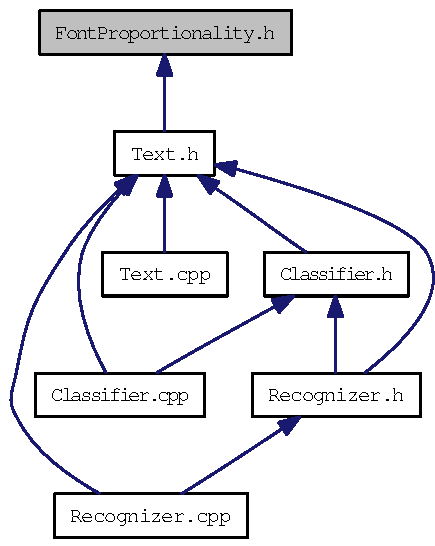
\includegraphics[width=122pt]{_font_proportionality_8h__dep__incl}
\end{center}
\end{figure}
\subsection*{Enumerations}
\begin{CompactItemize}
\item 
enum \hyperlink{_font_proportionality_8h_a9aa255df24db58a9b4cbc46941f2ac1}{FontProportionality} \{ \hyperlink{_font_proportionality_8h_a9aa255df24db58a9b4cbc46941f2ac1dc1e8f9aeb4699a239362b100670de62}{FONT\_\-MONOSPACED}, 
\hyperlink{_font_proportionality_8h_a9aa255df24db58a9b4cbc46941f2ac1923ae135c613560cceef2568bd9cfa8d}{FONT\_\-PROPORTIONAL}
 \}
\begin{CompactList}\small\item\em Font proportionality of a character. \item\end{CompactList}\end{CompactItemize}


\subsection{Enumeration Type Documentation}
\hypertarget{_font_proportionality_8h_a9aa255df24db58a9b4cbc46941f2ac1}{
\index{FontProportionality.h@{FontProportionality.h}!FontProportionality@{FontProportionality}}
\index{FontProportionality@{FontProportionality}!FontProportionality.h@{FontProportionality.h}}
\subsubsection[FontProportionality]{\setlength{\rightskip}{0pt plus 5cm}enum {\bf FontProportionality}}}
\label{_font_proportionality_8h_a9aa255df24db58a9b4cbc46941f2ac1}


Font proportionality of a character. 

This enumeration represents the different types of font proportionality that a text may have. The monospaced type is usual in fixed width fonts, while proportional type is usual in Roman fonts.

\begin{Desc}
\item[Author:]Eliezer Talón (\href{mailto:elitalon@gmail.com}{\tt elitalon@gmail.com}) \end{Desc}
\begin{Desc}
\item[Date:]2008-09-23 \end{Desc}
\begin{Desc}
\item[Enumerator: ]\par
\begin{description}
\index{FONT\_\-MONOSPACED@{FONT\_\-MONOSPACED}!FontProportionality.h@{FontProportionality.h}}\index{FontProportionality.h@{FontProportionality.h}!FONT\_\-MONOSPACED@{FONT\_\-MONOSPACED}}\item[{\em 
\hypertarget{_font_proportionality_8h_a9aa255df24db58a9b4cbc46941f2ac1dc1e8f9aeb4699a239362b100670de62}{
FONT\_\-MONOSPACED}
\label{_font_proportionality_8h_a9aa255df24db58a9b4cbc46941f2ac1dc1e8f9aeb4699a239362b100670de62}
}]In fixed width fonts. \index{FONT\_\-PROPORTIONAL@{FONT\_\-PROPORTIONAL}!FontProportionality.h@{FontProportionality.h}}\index{FontProportionality.h@{FontProportionality.h}!FONT\_\-PROPORTIONAL@{FONT\_\-PROPORTIONAL}}\item[{\em 
\hypertarget{_font_proportionality_8h_a9aa255df24db58a9b4cbc46941f2ac1923ae135c613560cceef2568bd9cfa8d}{
FONT\_\-PROPORTIONAL}
\label{_font_proportionality_8h_a9aa255df24db58a9b4cbc46941f2ac1923ae135c613560cceef2568bd9cfa8d}
}]In Roman fonts. \end{description}
\end{Desc}



Definition at line 20 of file FontProportionality.h.
\hypertarget{_font_weight_8h}{
\section{FontWeight.h File Reference}
\label{_font_weight_8h}\index{FontWeight.h(111)@{FontWeight.h(111)}}
}


\subsection{Detailed Description}


Definition in file \hyperlink{_font_weight_8h-source}{FontWeight.h}.

\subsection*{Enumerations}
\begin{CompactItemize}
\item 
enum \hyperlink{_font_weight_8h_ecff23ba4a68486421bcea57e095fe66}{FontWeight} \{ \par
\hyperlink{_font_weight_8h_ecff23ba4a68486421bcea57e095fe6650d1448013c6f17125caee18aa418af7}{NORMAL}, 
\hyperlink{_font_weight_8h_ecff23ba4a68486421bcea57e095fe6639fc1130a1e2c8f8c1ad3deee8c0c5dc}{BOLD}, 
\hyperlink{_font_weight_8h_ecff23ba4a68486421bcea57e095fe66c1005585401f6364dc82967ecf313617}{ITALIC}, 
\hyperlink{_font_weight_8h_ecff23ba4a68486421bcea57e095fe66d460ec31770f376d61ffb3a9b0b31990}{UNDERLINED}, 
\par
\hyperlink{_font_weight_8h_ecff23ba4a68486421bcea57e095fe66a38b4c4aaa3055986332429724296b82}{BOLD\_\-ITALIC}, 
\hyperlink{_font_weight_8h_ecff23ba4a68486421bcea57e095fe662cbda7343b95170af5caffae74aac09b}{BOLD\_\-UNDERLINED}, 
\hyperlink{_font_weight_8h_ecff23ba4a68486421bcea57e095fe665505c1f3544235b341e632fd0c73bbd0}{ITALIC\_\-UNDERLINED}
 \}
\begin{CompactList}\small\item\em Font weight of a character. \item\end{CompactList}\end{CompactItemize}


\subsection{Enumeration Type Documentation}
\hypertarget{_font_weight_8h_ecff23ba4a68486421bcea57e095fe66}{
\index{FontWeight.h@{FontWeight.h}!FontWeight@{FontWeight}}
\index{FontWeight@{FontWeight}!FontWeight.h@{FontWeight.h}}
\subsubsection[FontWeight]{\setlength{\rightskip}{0pt plus 5cm}enum {\bf FontWeight}}}
\label{_font_weight_8h_ecff23ba4a68486421bcea57e095fe66}


Font weight of a character. 

This enumeration represents the different types of font weight that a character may have. All the possible combinations are present, though in a normal text the most common are the three first font weights: bold, italic and normal.

\begin{Desc}
\item[Author:]Eliezer Talón (\href{mailto:elitalon@gmail.com}{\tt elitalon@gmail.com}) \end{Desc}
\begin{Desc}
\item[Date:]2008-09-18 \end{Desc}
\begin{Desc}
\item[Enumerator: ]\par
\begin{description}
\index{NORMAL@{NORMAL}!FontWeight.h@{FontWeight.h}}\index{FontWeight.h@{FontWeight.h}!NORMAL@{NORMAL}}\item[{\em 
\hypertarget{_font_weight_8h_ecff23ba4a68486421bcea57e095fe6650d1448013c6f17125caee18aa418af7}{
NORMAL}
\label{_font_weight_8h_ecff23ba4a68486421bcea57e095fe6650d1448013c6f17125caee18aa418af7}
}]Normal font, without decorations. \index{BOLD@{BOLD}!FontWeight.h@{FontWeight.h}}\index{FontWeight.h@{FontWeight.h}!BOLD@{BOLD}}\item[{\em 
\hypertarget{_font_weight_8h_ecff23ba4a68486421bcea57e095fe6639fc1130a1e2c8f8c1ad3deee8c0c5dc}{
BOLD}
\label{_font_weight_8h_ecff23ba4a68486421bcea57e095fe6639fc1130a1e2c8f8c1ad3deee8c0c5dc}
}]Only bold. \index{ITALIC@{ITALIC}!FontWeight.h@{FontWeight.h}}\index{FontWeight.h@{FontWeight.h}!ITALIC@{ITALIC}}\item[{\em 
\hypertarget{_font_weight_8h_ecff23ba4a68486421bcea57e095fe66c1005585401f6364dc82967ecf313617}{
ITALIC}
\label{_font_weight_8h_ecff23ba4a68486421bcea57e095fe66c1005585401f6364dc82967ecf313617}
}]Only italic. \index{UNDERLINED@{UNDERLINED}!FontWeight.h@{FontWeight.h}}\index{FontWeight.h@{FontWeight.h}!UNDERLINED@{UNDERLINED}}\item[{\em 
\hypertarget{_font_weight_8h_ecff23ba4a68486421bcea57e095fe66d460ec31770f376d61ffb3a9b0b31990}{
UNDERLINED}
\label{_font_weight_8h_ecff23ba4a68486421bcea57e095fe66d460ec31770f376d61ffb3a9b0b31990}
}]Normal but underlined. \index{BOLD\_\-ITALIC@{BOLD\_\-ITALIC}!FontWeight.h@{FontWeight.h}}\index{FontWeight.h@{FontWeight.h}!BOLD\_\-ITALIC@{BOLD\_\-ITALIC}}\item[{\em 
\hypertarget{_font_weight_8h_ecff23ba4a68486421bcea57e095fe66a38b4c4aaa3055986332429724296b82}{
BOLD\_\-ITALIC}
\label{_font_weight_8h_ecff23ba4a68486421bcea57e095fe66a38b4c4aaa3055986332429724296b82}
}]Both bold and italic. \index{BOLD\_\-UNDERLINED@{BOLD\_\-UNDERLINED}!FontWeight.h@{FontWeight.h}}\index{FontWeight.h@{FontWeight.h}!BOLD\_\-UNDERLINED@{BOLD\_\-UNDERLINED}}\item[{\em 
\hypertarget{_font_weight_8h_ecff23ba4a68486421bcea57e095fe662cbda7343b95170af5caffae74aac09b}{
BOLD\_\-UNDERLINED}
\label{_font_weight_8h_ecff23ba4a68486421bcea57e095fe662cbda7343b95170af5caffae74aac09b}
}]Both bold and underlined. \index{ITALIC\_\-UNDERLINED@{ITALIC\_\-UNDERLINED}!FontWeight.h@{FontWeight.h}}\index{FontWeight.h@{FontWeight.h}!ITALIC\_\-UNDERLINED@{ITALIC\_\-UNDERLINED}}\item[{\em 
\hypertarget{_font_weight_8h_ecff23ba4a68486421bcea57e095fe665505c1f3544235b341e632fd0c73bbd0}{
ITALIC\_\-UNDERLINED}
\label{_font_weight_8h_ecff23ba4a68486421bcea57e095fe665505c1f3544235b341e632fd0c73bbd0}
}]Both italic and underlined. \end{description}
\end{Desc}



Definition at line 18 of file FontWeight.h.
\hypertarget{_word_rate_8h}{
\section{WordRate.h File Reference}
\label{_word_rate_8h}\index{WordRate.h(125)@{WordRate.h(125)}}
}


\subsection{Detailed Description}
Declaration of custom type WordRate. 



Definition in file \hyperlink{_word_rate_8h-source}{WordRate.h}.

{\tt \#include $<$utility$>$}\par
{\tt \#include $<$string$>$}\par


Include dependency graph for WordRate.h:\nopagebreak
\begin{figure}[H]
\begin{center}
\leavevmode
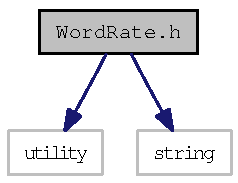
\includegraphics[width=75pt]{_word_rate_8h__incl}
\end{center}
\end{figure}


This graph shows which files directly or indirectly include this file:\nopagebreak
\begin{figure}[H]
\begin{center}
\leavevmode
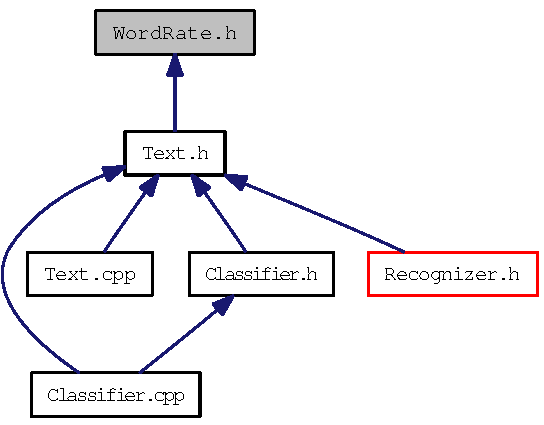
\includegraphics[width=148pt]{_word_rate_8h__dep__incl}
\end{center}
\end{figure}
\subsection*{Typedefs}
\begin{CompactItemize}
\item 
typedef std::pair$<$ std::string, unsigned int $>$ \hyperlink{_word_rate_8h_8cfef8793106ac45a83059bd5573cbb3}{WordRate}
\begin{CompactList}\small\item\em Appearance rate of a word. \item\end{CompactList}\end{CompactItemize}


\subsection{Typedef Documentation}
\hypertarget{_word_rate_8h_8cfef8793106ac45a83059bd5573cbb3}{
\index{WordRate.h@{WordRate.h}!WordRate@{WordRate}}
\index{WordRate@{WordRate}!WordRate.h@{WordRate.h}}
\subsubsection[WordRate]{\setlength{\rightskip}{0pt plus 5cm}typedef std::pair$<$std::string, unsigned int$>$ {\bf WordRate}}}
\label{_word_rate_8h_8cfef8793106ac45a83059bd5573cbb3}


Appearance rate of a word. 

This pair keeps the number of appearances of a word in a text

\begin{Desc}
\item[Author:]Eliezer Talón (\href{mailto:elitalon@gmail.com}{\tt elitalon@gmail.com}) \end{Desc}
\begin{Desc}
\item[Date:]2008-09-19 \end{Desc}


Definition at line 21 of file WordRate.h.
\printindex
\end{document}
